\documentclass[
    ngerman,
    authorontitle=true,
]{bfhbeamer}

%\usepackage[main=ngerman]{babel}

% Der folgende Block ist nur bei pdfTeX auf Versionen vor April 2018 notwendig
\usepackage{iftex}
\ifPDFTeX
\usepackage[utf8]{inputenc}%kompatibilität mit TeX Versionen vor April 2018
\fi
\usepackage{bytefield}
\usepackage{amssymb}
\usepackage{pifont}
\usepackage{xcolor}
\usepackage{fontawesome5}
\usepackage{todonotes}
\usepackage{hyperref}
\usepackage{graphicx}
\usepackage{svg}
\svgsetup{inkscapelatex=false}
\usepackage{subfigure}
\usepackage{tikz}
\usetikzlibrary{positioning}
\usepackage{tabto}

%Makros für Formatierungen der Doku
%Im Allgemeinen nicht notwendig!
\let\code\texttt

\title{Gitterprobleme \& LWE (Learning with errors)}
\subtitle{BZE1315 Zufallsgesteurte Algorithmen - Post-Quanten Kryptographie}
\author[]{Lukas von Allmen - vonal3@bfh.ch}
\institute{Bern University of Applied Sciences}
\titlegraphic*{\includegraphics{{../assets/title_graphics.png}}}

%Activate the output of a frame number:
\setbeamertemplate{section page}[BFH-ruled]
\setbeamertemplate{page number in head/foot}[framenumber]
\setbeameroption{show notes on second screen=bottom}

\begin{document}

\setbeamertemplate{title page}[BFH-graphic]
\maketitle

\section{Einleitung}\label{sec:introduction}
\begin{frame}{Rückblick~\textendash~Problemstellung}
    \begin{itemize}
        \item Einführung in Quanten-Computing
        \item Problem von Deutsch \& Deutsch-Jozsa-Algorithmus
        \item Starke indizien für Quantenüberlegenheit (Quantum Supremacy)
        \item Shor's-Algorithmus
        \item \textbf{Was nun?}
    \end{itemize}

    \note{
        Quantenüberlegenheit: Quantencomputer schlägt klassische Rechner in spezifischen Aufgaben - jedoch noch nicht eindeutig bewiesen.\newline
        \newline
        Wenn ein Quantencomputer gebaut werden kann um Shor's-Algorithmus effektiv laufen zu lassen, können klassische Verschlüsselungssysteme welche auf der Primfaktorzerlegung basieren einfach geknackt werden (e.g., RSA, ECC).
    }
\end{frame}

\begin{frame}{Entwicklung quanten-resistenter Einwegfunktionen}
    \begin{itemize}
        \item {
            \textbf{Learning with Errors (LWE)~\&~Gitterprobleme}\newline
            \(\rightarrow\) mutmasslich NP-Schwer~\&~quanten-resistent
        }
        \item \textbf{Verfahren von Regev} (Odded Regev)
        \item Cryptographic Suite for Algebraic Lattices (CRYSTALS) Projekt
        \item CRYSTALS entwickelt \textbf{Kyber} (Verschlüsselung)~\&~Dilithium (Signaturen)
        \item Module-Lattice-Based Key-Encapsulation Mechanism (ML-KEM)
    \end{itemize}

    \note{
        Es stellt sich heraus, dass sich dazu Learning with Errors (LWE) in kombination mit Gitterprblemen eignet.\newline
        \newline
        Diese Methode wurde 2005 erstmals von Odded Regev verwendet, um ein Quanten-Resistentes Verschlüsselungsverfahren zu entwerfen. 2018 erhielt Regev für diese Arbeit den Gödel-Preis.\newline
        \newline
        Das Verfahren wurde im Projekt CRYSTALS von einem Kryptografen-Team unter dem Namen "Kyber" weiterentwickelt und erstmals 2017 veröffentlicht.\newline
        \newline
        Kyber wurde von der NIST standartisiert und 2024 unter dem Namen Module-Lattice-Based Key-Encapsulation Mechanism (kruz: ML-KEM) veröffentlicht.\newline
    }
\end{frame}


\begin{frame}{Übersicht}
    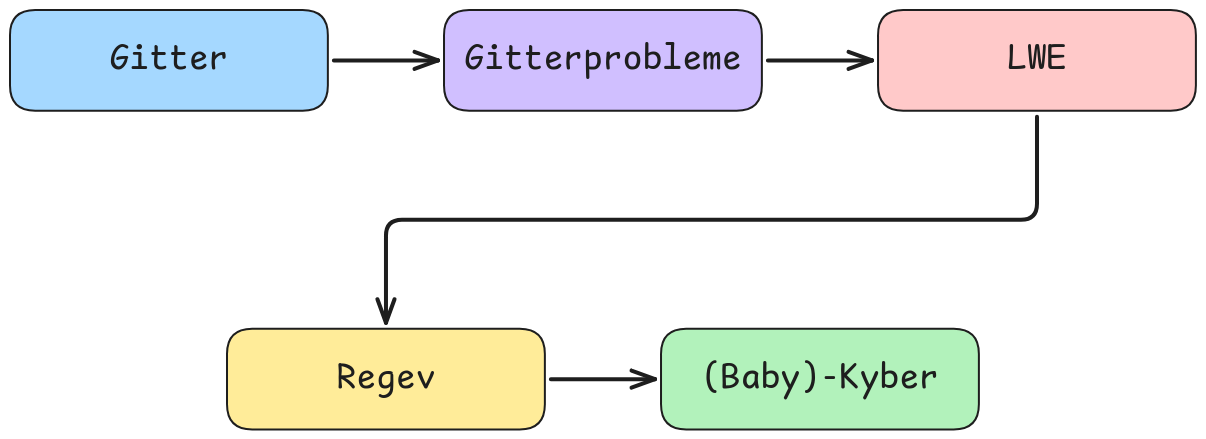
\includegraphics[width=\textwidth]{../assets/postquantum_lectures_overview.excalidraw.png}
    \note{
        In diesem Vortrag erarbeiten wir die mathematischen Grundlagen zum Verstehen von Gitterproblemen, Learning with Errors und wie man aus ihnen ein Verschlüsselungssystem entwerfen kann.\newline
        \newline
        Im nächsten Vortag schauen wir uns das Verfahren von Regev und Baby-Kyber an, eine vereinfachte Version von Kyber.
    }
\end{frame}

\section{Mathematische Gitter}\label{sec:lattices}
\begin{frame}{Definition Gitter (Lattices)}
    \begin{definition}[Gitter]
        Sei $B = \{\mathbf{b}_1, \mathbf{b}_2, \dots, \mathbf{b}_m\}$ eine Menge linear unabhängiger Vektoren aus dem euklidischen Vektorraum $\mathbb{R}^n$. Dann heisst die Menge aller ganzzahligen Linearkombinationen
        \[
            \mathcal{L}(B) = \left\{ \sum_{i=1}^{m} a_i \mathbf{b}_i \;\middle|\; a_i \in \mathbb{Z} \right\} \subseteq \mathbb{R}^n
        \]
        das von $B$ erzeugte \textbf{Gitter} in $\mathbb{R}^n$. $B$ nennen wir die \textbf{Basis} des Gitters $\mathcal{L}$.
    \end{definition}
\end{frame}

\begin{frame}{Auffrischung: Euklidische Vektorräume}
    \begin{itemize}
        \item
    \end{itemize}
\end{frame}

\begin{frame}{Auffrischung: Lineare Unabhängigkeit}
    \begin{itemize}
        \item
    \end{itemize}
\end{frame}

\begin{frame}{Auffrischung: Linear Kombinationen}
    \begin{itemize}
        \item
    \end{itemize}
\end{frame}

\begin{frame}{Gitter als Matritze}
    \begin{itemize}
        \item Ein Gitter kann äquivalent aus einer Matrix $\mathbf{B}$ erzeugt werden, deren Spaltenvektoren die Basisvektoren sind:
        $\mathcal{L}(\mathbf{B}) = \{\mathbf{B}\mathbf{a} \mid \mathbf{a} \in \mathbb{Z}^m\}$
    \end{itemize}
\end{frame}


\section{Gitterprobleme}\label{sec:lattice_problems}
\begin{frame}{Beispiel für ein einfaches Gitterproblem}
    \textbf{Problemstellung:}
    \begin{itemize}
        \item Sei $\mathbf{g}_1, \dots, \mathbf{g}_k \in \mathbb{R}^n$ ein Set von Vektoren welche das Gitter $\mathcal{L}$ generieren
        \item Berechne eine Basis von $\mathbf{b}_1, \dots, \mathbf{b}_m \in \mathbb{R}^n$ von $\mathcal{L}$
        \item Bestimme, ob ein beliebiger Vektor ein Element vom Gitter $\mathcal{L}$ ist
    \end{itemize}
    \textbf{Lösungsansatz:}
    \begin{itemize}
        \item Basismatrize $\mathbf{B}$ mit dem Gauss-Algorithmus aus den $\mathbf{g}_i$ berechnen
        \item Das lineare Gleichungssystem lösen
        \item Der Vektor $\mathbf{c}$ ist genau dann ein Element von $\mathcal{L}$, wenn $\mathbf{x} \in \mathbb{Z}^m$ ist (alle Einträge ganzzahlig)
    \end{itemize}
    \note{
        Wieso ist das so? Das Gitter $\mathcal{L}$ besteht per Definition genau aus allen ganzzahligen Linearkombinationen der Basisvektoren,
        also $\mathcal{L} = \{\mathbf{B}\mathbf{x} : \mathbf{x} \in \mathbb{Z}^m\}$.
        Ein Vektor $\mathbf{c}$ liegt also genau dann im Gitter, wenn es ganzzahlige Koeffizienten $x_i$ gibt mit $\mathbf{c} = \mathbf{B}\mathbf{x}$.\newline
        \newline
        Nur wenn Fragen auftauchen:\newline
        Da die Basisvektoren linear unabhängig sind, hat das Gleichungssystem $\mathbf{B}\mathbf{x} = \mathbf{c}$ höchstens eine Lösung (über $\mathbb{R}$).
        Es gibt also keine andere Darstellung von $\mathbf{c}$, die ganzzahlig sein könnte, falls die berechnete Lösung nicht ganzzahlig ist.
        Ist $\mathbf{x}$ ganzzahlig, gilt $\mathbf{c} \in \mathcal{L}$, sonst $\mathbf{c} \notin \mathcal{L}$.\newline
    }
\end{frame}

\begin{frame}{Einfaches Gitterproblem: Beispiel mit Lösung}
    \textbf{Gegeben:}
    \[
        \mathbf{g}_1 = \begin{pmatrix} 2 \\ 0 \end{pmatrix},\;
        \mathbf{g}_2 = \begin{pmatrix} 1 \\ 2 \end{pmatrix},\;
        \mathbf{g}_3 = \begin{pmatrix} 3 \\ 2 \end{pmatrix}
        \qquad
        \qquad
        \mathbf{c}_1 = \begin{pmatrix} 5 \\ 2 \end{pmatrix},\;
        \mathbf{c}_2 = \begin{pmatrix} 4 \\ 2 \end{pmatrix}
    \]
    \textbf{Lösung:}
    \begin{itemize}
        \item Basis: $\mathbf{g}_3 = \mathbf{g}_1 + \mathbf{g}_2$ ist linear abhängig, also weglassen:
        $\mathbf{B} = \begin{pmatrix} 2 & 1 \\ 0 & 2 \end{pmatrix}$
        \item $\mathbf{c}_1$: $x_2 = 1$, $x_1 = 2$ \qquad also $\mathbf{x} = \begin{pmatrix} 2 \\ 1 \end{pmatrix} \in \mathbb{Z}^2$ \; $\Rightarrow$ $\mathbf{c}_1 \in \mathcal{L}$
        \item $\mathbf{c}_2$: $x_2 = 1$, $x_1 = \tfrac{3}{2}$ \qquad also $\mathbf{x} \notin \mathbb{Z}^2$ \; $\Rightarrow$ $\mathbf{c}_2 \notin \mathcal{L}$
    \end{itemize}
    \note{
        Laufzeit: Das Verfahren ist polynomiell, bei $k \approx n$ Erzeugern etwa $O(n^3)$ (Basisberechnung dominiert, Gleichungssystem lösen ist $O(n \cdot m^2)$).\newline
    }
\end{frame}

\begin{frame}{Shortest Vector Problem (SVP)~\textendash~... des kürzesten Vektors}
    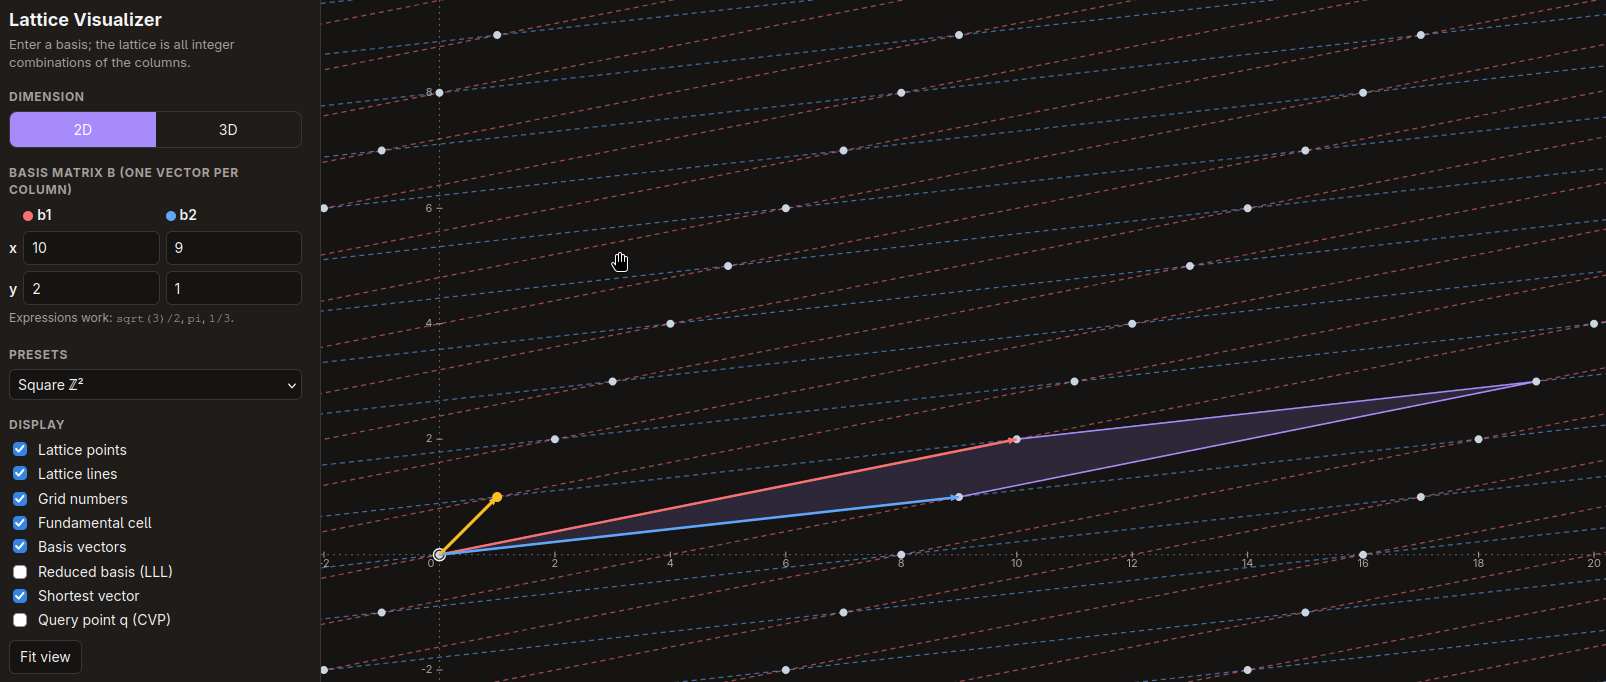
\includegraphics[width=\textwidth]{../assets/lattice_tool_shortest_vector_problem.png}
    \note{
        Vereinfacht gesagt beschreibt das Problem des kürzesten Vektors (kurz SVP) die Suche nach dem Vektor mit der kürzesten Distanz zum Nullpunkt/Uhrsprung.
    }
\end{frame}

\begin{frame}{Shortest Vector Problem (SVP): Definition}
    \begin{itemize}
        \item Sei $\mathcal{L}$ ein Gitter mit einer Basis $\mathbf{B} \in \mathbb{R}^{n \times m}$ und einer Norm $\|\cdot\|$.
        \item Sei $\lambda(\mathcal{L})$ die Länge des kürzesten Vektors ungleich null in $\mathcal{L}$.
        \item Die Aufgabe, ein $\mathbf{l} \in \mathcal{L}$ zu finden mit $\|\mathbf{l}\| = \lambda(\mathcal{L})$, also irgendeinen kürzesten Vektor von $\mathcal{L}$ zu finden, heisst \textit{Shortest Vector Problem (SVP)}.
    \end{itemize}
    \vspace{2em}
    {\setbeamerfont{itemize/enumerate body}{size=\footnotesize}
    \begin{itemize}
        \item NP-Schwer: z.B. Enumeration $2^{O(n \log n)}$
        \item LLL findet in polynomieller Zeit ein Resultat, dass max. $2^{O(n)}$ zu lang ist
    \end{itemize}
    }
    \note{
        SVP ist NP-schwer und exakte Algorithmen brauchen exponentielle Zeit in der Dimension $n$: Also etwas in der Form $2^{O(n \log n)}$, z.B. für die Enumeration.\newline
        \newline
        In polynomieller Zeit ist nur eine Näherung möglich: LLL findet einen Vektor, der höchstens um einen Faktor $2^{O(n)}$ länger ist als der kürzeste.
    }
\end{frame}

\begin{frame}{Closest Vector Problem (CVP)~\textendash~... des nächstgelegenen Vektors}
    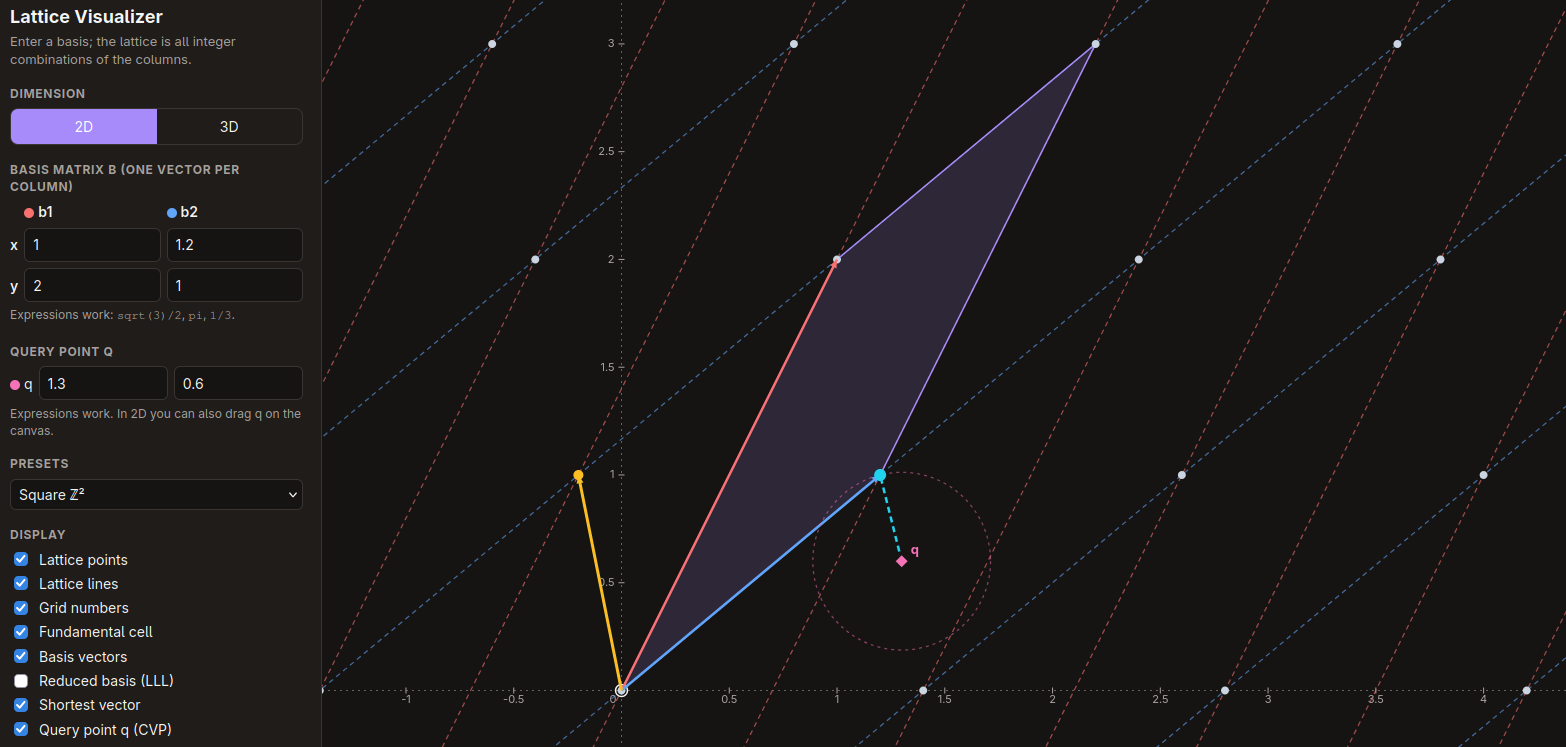
\includegraphics[width=\textwidth]{../assets/lattice_tool_closest_vector_problem.png}
    \note{
        Die Suche nach dem Vektor mit der kürzesten Distanz zu einem beliebig gewählten Punkt nennt man das Problem des nächstgelegenen Vektors (kurz CVP).
    }
\end{frame}

\begin{frame}{Closest Vector Problem (CVP): Definition}
    \begin{itemize}
        \item Sei $\mathcal{L}$ ein Gitter mit einer Basis $\mathbf{B} \in \mathbb{R}^{n \times m}$ und einer Norm $\|\cdot\|$ (Vektorlänge, üblicherweise die Euklidische Norm $\|\mathbf{v}\| = \sqrt{v_1^2 + \dots + v_n^2}$).
        \item Gegeben sei ein $\mathbf{q} \in \mathbb{R}^n$.
        \item Die Aufgabe, ein $\mathbf{l} \in \mathcal{L}$ zu finden, für das $\|\mathbf{l} - \mathbf{q}\|$ minimal ist, also den Gittervektor $\mathbf{l}$ zu finden, der einem beliebig vorgegebenen Vektor am nächsten liegt, heisst \textit{Closest Vector Problem (CVP)}.
    \end{itemize}
    \vspace{2em}
    {\setbeamerfont{itemize/enumerate body}{size=\footnotesize}
    \begin{itemize}
        \item NP-Schwer: mindestens so schwer wie SVP
        \item Babai-Algorithmus findet in polynomieller Zeit ein Resultat, dass max. $2^{O(n)}$ zu lang ist
    \end{itemize}
    }
    \note{
        Zur Geschätzte Laufzeit: CVP ist NP-schwer und gilt als mindestens so schwer wie SVP.\newline
        \newline
        In polynomieller Zeit geht nur eine Näherung, z.B. der Babai-Algorithmus auf einer LLL-reduzierten Basis mit einem Faktor $2^{O(n)}$.
    }
\end{frame}

\section{LWE (Learning with errors)}\label{sec:learning_with_errors}
\begin{frame}{Auffrischung: Ring}
    \begin{itemize}
        \item Ein \textbf{Ring} ist eine Menge $R$ mit Addition $+$ und Multiplikation $\cdot$
        \item Addieren, subtrahieren und multiplizieren ist immer möglich (mit $0$, $1$ und Gegenelementen)
        \item Distributivgesetz: $a \cdot (b + c) = a \cdot b + a \cdot c$
        \item Division ist nicht immer möglich (sonst wäre es ein Körper)
        \item \textbf{Beispiele:}
        \begin{itemize}
            \item die ganzen Zahlen $\mathbb{Z}$
            \item $\mathbb{Z}_q$: ganze Zahlen modulo $q$, wie eine Uhr mit $q$ Stunden, z.B. in $\mathbb{Z}_7$ gilt $5 + 4 = 2$
        \end{itemize}
    \end{itemize}
    \note{
        Für LWE ist der Ring $\mathbb{Z}_q$ wichtig: Man rechnet mit ganzen Zahlen und nimmt nach jeder Operation den Rest modulo $q$.\newline
        \newline
        Ring vs. Gruppe: Eine Gruppe hat nur \emph{eine} Operation (z.B. $+$) mit neutralem Element und Inversen.
        Ein Ring hat zwei: $(R, +)$ ist eine kommutative Gruppe, dazu kommt die Multiplikation, verbunden über das Distributivgesetz.
        Im Ring gibt es nicht zu jedem Element ein multiplikatives Inverses, deshalb ist Division nicht immer möglich.\newline
        \newline
        Körper vs. Ring: Jeder Körper ist ein Ring, in dem zusätzlich jedes Element außer $0$ ein multiplikatives Inverses hat. Beispiele: $\mathbb{Q}$, $\mathbb{R}$, $\mathbb{Z}_p$ für eine Primzahl $p$.
        $\mathbb{Z}$ ist ein Ring, aber kein Körper. Also: Gruppe $\leftarrow$ Ring $\leftarrow$ Körper.
    }
\end{frame}

\begin{frame}{Einführung in Learning with Errors (LWE)}
    Sei $\mathbb{Z}_q = \mathbb{Z}/q\mathbb{Z}$ der Ring der ganzen Zahlen modulo $q$, also die Menge der ganzen Zahlen kleiner
    als $q$ mit den Operationen $+$ und $\cdot$ modulo $q$.\newline`
    Als lineares Gleichungssystem:
    \[
        \mathbf{A} \cdot \mathbf{s} = \mathbf{b},
    \]
    wobei $\mathbf{A} \in \mathbb{Z}_q^{n \times m}$, $\mathbf{s} \in \mathbb{Z}_q^{m}$ und $\mathbf{b} \in \mathbb{Z}_q^{n}$.
    \newline
    \newline
    \centering
    Zum Beispiel:
    \[
        \underbrace{\begin{pmatrix}
            10 & 3 & 5 & 1 \\
            4  & 1 & 1 & 2 \\
            \vdots & \vdots & \vdots & \vdots \\
            3  & 1 & 1 & 5
        \end{pmatrix}}_{\mathbf{A}}
        \cdot
        \underbrace{\begin{pmatrix}
            s_1 \\ s_2 \\ s_3 \\ s_4
        \end{pmatrix}}_{\mathbf{s}}
        =
        \underbrace{\begin{pmatrix}
            10 \\ 3 \\ \vdots \\ 8
        \end{pmatrix}}_{\mathbf{b}}
    \]
    \note{

    }
\end{frame}

\begin{frame}{Einführung in Learning with Errors (LWE)}
    Als Gleichungssystem:
    \begin{align*}
        10 \cdot s_1 + 3 \cdot s_2 + 5 \cdot s_3 + 1 \cdot s_4 &= 10 \\
        4 \cdot s_1 + 1 \cdot s_2 + 1 \cdot s_3 + 2 \cdot s_4 &= 3 \\
        &\;\;\vdots \\
        3 \cdot s_1 + 1 \cdot s_2 + 1 \cdot s_3 + 5 \cdot s_4 &= 8
    \end{align*}

    Fügt man kleine Fehlerwerte $\mathbf{e} \in \mathbb{Z}_q^{n}$ ein, erhält man
    \[
        \mathbf{A} \cdot \mathbf{s} + \mathbf{e} = \mathbf{b},
    \]
    was das Lösen des Gleichungssystems überraschend schwer macht.
    \note{
        Dies liegt an der Verbindung zu den oben beschriebenen schweren Gitterproblemen.
    }
\end{frame}

\begin{frame}{LWE-Beispiel: ohne Fehler}
    Wähle $q = 17$, $n = 4$ Gleichungen, $m = 2$ Unbekannte und das Secret $\mathbf{s} = (3, 5)^T$ (geheim).
    \[
        \underbrace{\begin{pmatrix}
            9 & 8 \\ 4 & 2 \\ 7 & 11 \\ 6 & 9
        \end{pmatrix}}_{\mathbf{A}}
        \cdot
        \begin{pmatrix} s_1 \\ s_2 \end{pmatrix}
        =
        \underbrace{\begin{pmatrix} 16 \\ 5 \\ 8 \\ 12 \end{pmatrix}}_{\mathbf{b}}
        \bmod 17
    \]
    \begin{itemize}
        \item Zwei Gleichungen genügen: Gauss-Algorithmus liefert $\mathbf{s} = (3, 5)^T$
        \item Kontrolle, z.B. Gleichung 3: $7 \cdot 3 + 11 \cdot 5 = 76 = 8 \bmod 17$
    \end{itemize}
    \note{
        Ohne Fehler ist das ein ganz normales lineares Gleichungssystem, nur dass man modulo $17$ rechnet.
        Aus den ersten beiden Gleichungen ergibt sich das Secret mit dem Gauss-Algorithmus. Die Determinante $9 \cdot 2 - 8 \cdot 4 = -14 = 3 \bmod 17$ ist invertierbar, deshalb ist die Lösung eindeutig.
    }
\end{frame}

\begin{frame}{LWE-Beispiel: mit Fehler}
    Gleiche Daten, aber mit geheimem kleinem Fehler $\mathbf{e} = (1, -1, 1, 0)^T$. Öffentlich: $(\mathbf{A}, \mathbf{b})$, geheim: $\mathbf{s}$, $\mathbf{e}$.
    \[
        \mathbf{A} \cdot \mathbf{s} + \mathbf{e} = \mathbf{b},
        \qquad
        \mathbf{b} = (0, 4, 9, 12)^T \bmod 17
    \]
    \begin{itemize}
        \item Gauss mit den ersten beiden Gleichungen liefert $(12, 12)^T$
        \item {
            Falsch: Gleichung 3 ergibt $7 \cdot 12 + 11 \cdot 12 = 12 \neq 9$
            \newline
            \(\rightarrow\) das Gleichungssystem hat keine exakte Lösung mehr
        }
        \item {
            Gesucht: das $\mathbf{s}$, bei dem $\mathbf{b} - \mathbf{A} \cdot \mathbf{s}$ nur kleine Einträge hat
            \newline
            \(\rightarrow\) alle $17^2 = 289$ Kandidaten probieren: nur $(3, 5)^T$ passt
        }
        \item Kyber-768: $m = 768$, $q = 3329$ $\Rightarrow$ $3329^{768} \approx 10^{2705}$ Kandidaten
    \end{itemize}
    \note{
        Der Fehler macht das System inkonsistent: Zwei beliebige Gleichungen liefern eine Lösung, die zu den anderen Gleichungen nicht passt.
        Man müsste also erraten, welche Gleichungen wie stark verfälscht sind.\newline
        \newline
        Bei diesem Spielzeugbeispiel gibt es genau ein $\mathbf{s}$, bei dem alle Reste $\mathbf{b} - \mathbf{A}\mathbf{s}$ im Bereich $\{-1, 0, 1\}$ liegen, nämlich $(3, 5)^T$ mit Rest $\mathbf{e} = (1, -1, 1, 0)^T$.
        Das ist genau die Idee von CVP: der Gitterpunkt $\mathbf{A}\mathbf{s}$, der $\mathbf{b}$ am nächsten liegt.
        Bei realen Parametern ist die Suche nach diesem Punkt zu aufwendig.\newline
        \newline
        Kyber-768 hat ein Secret mit $m = 768$ Einträgen in $\mathbb{Z}_{3329}$. Das sind $3329^{768} \approx 10^{2705}$ (etwa $2^{8986}$) Kandidaten. Zum Vergleich: Das sichtbare Universum enthält etwa $10^{80}$ Atome.\newline
        Selbst wenn man ausnutzt, dass die Einträge des Secrets bei Kyber klein sind (hier aus $\{-2, \dots, 2\}$), bleiben $5^{768} \approx 10^{537}$ Möglichkeiten.
    }
\end{frame}

\begin{frame}{Decisional LWE (dLWE)}
    \[
        \mathbf{A} \cdot \mathbf{s} + \mathbf{e} = \mathbf{b},
    \]
    \begin{itemize}
        \item Das LWE-Problem kann als Entscheidungsproblem ausgelegt werden
        \item Gegeben ist eine LWE-Aufgabe $(\mathbf{A}, \mathbf{b})$, wobei $\mathbf{s}$ und $\mathbf{e}$ geheim sind
        \item {
            Die Aufgabe ist es zu erraten, ob die Werte von $\mathbf{b}$ (gleich schwer)
            \begin{itemize}
                \item als $\mathbf{A} \cdot \mathbf{s} + \mathbf{e}$ berechnet wurden
                \item oder zufällig gewählt wurden
            \end{itemize}
        }
        \item Oded Regev hat die Reduktion von LWE auf dLWE bewiesen
    \end{itemize}
    \note{
        Warum ist das relevant? Bei einem Verschlüsselungssystem reicht es nicht, dass der Angreifer das Secret nicht finden kann.
        Der Chiffretext darf ihm auch sonst keine Information über die Nachricht verraten. Ein Chiffretext, der sich von Zufall nicht unterscheiden lässt, verrät nichts.\newline
        \newline
        Wie zeigt das die Sicherheit? Ist dLWE schwer, sind echte LWE-Daten $(\mathbf{A}, \mathbf{b})$ von rein zufälligen Daten nicht zu unterscheiden.
        Verschlüsselt man ein Bit, sieht der Chiffretext deshalb für einen Angreifer wie Zufall aus, egal ob eine 0 oder eine 1 darin steckt.
        Könnte er trotzdem das Bit erkennen, hätte er damit dLWE gelöst (Sicherheitsbeweis durch Reduktion).\newline
        \newline
        Weil LWE und dLWE gleich schwer sind (Regev), reicht es, die Schwere von LWE anzunehmen.
    }
\end{frame}

\begin{frame}{Verbindung zwischen LWE und Gitterproblemen: CVP}
    \[
        \mathbf{A} \cdot \mathbf{s} + \mathbf{e} = \mathbf{b},
    \]
    \begin{itemize}
       \item $\mathbf{A} \in \mathbb{Z}_q^{n \times m}$, $\mathbf{b} \in \mathbb{Z}_q^{n}$ und $\mathbf{s} \in \mathbb{Z}_q^{m}$, $\mathbf{e} \in \mathbb{Z}_q^{n}$ sind kleine Vektoren
       \item Eine konkrete LWE-Instanz lässt sich lösen, indem man das Closest Vector Problem löst
       \item Der nächstgelegene Gittervektor zu $\mathbf{b}$ ist fast immer der Gittervektor $\mathbf{A} \cdot \mathbf{s}$ mit Abstand $\mathbf{e}$
    \end{itemize}
    \note{
        Warum führt das auf CVP? Alle ganzzahligen Linearkombinationen der Spalten von $\mathbf{A}$ (modulo $q$) bilden ein Gitter. $\mathbf{A} \cdot \mathbf{s}$ ist ein Punkt dieses Gitters.
        Der Vektor $\mathbf{b} = \mathbf{A} \cdot \mathbf{s} + \mathbf{e}$ liegt aber leicht daneben, nämlich um den kleinen Fehler $\mathbf{e}$.
        Den Gitterpunkt zu finden, der $\mathbf{b}$ am nächsten liegt, ist genau das Closest Vector Problem. Weil $\mathbf{e}$ klein ist, ist dieser Punkt meistens $\mathbf{A} \cdot \mathbf{s}$, und daraus lässt sich $\mathbf{s}$ berechnen.
    }
\end{frame}

\begin{frame}{Verbindung zwischen LWE und Gitterproblemen: SVP}
    Sei $\mathcal{L}$ ein Gitter, $\parallel$ die Konkatenation und $\mathbf{I}_n$ die $n \times n$-Einheitsmatrize
    \[
        \mathcal{L} = \{\mathbf{x} \in \mathbb{Z}^{m+n+1} \mid (\mathbf{A} \parallel \mathbf{I}_n \parallel (-\mathbf{b})) \cdot \mathbf{x} = \mathbf{0} \bmod q\},
    \]
    Der Spaltenvektor $(\mathbf{s}, \mathbf{e}, 1)$ ist ein Element von $\mathcal{L}$, denn
    \[
        \begin{pmatrix} \mathbf{A} & \mathbf{I}_n & -\mathbf{b} \end{pmatrix}
        \cdot
        \begin{pmatrix} \mathbf{s} \\ \mathbf{e} \\ 1 \end{pmatrix}
        = \mathbf{A} \cdot \mathbf{s} + \mathbf{e} - \mathbf{b} = \mathbf{b} - \mathbf{b} = \mathbf{0} \bmod q.
    \]
    \note{
        Warum ist $(\mathbf{s}, \mathbf{e}, 1)$ ein kürzester Vektor? $\mathbf{s}$ und $\mathbf{e}$ sind klein, die letzte Komponente ist $1$, der Vektor ist also sehr kurz.
        Die meisten anderen Gittervektoren von $\mathcal{L}$ haben dagegen Einträge in der Grössenordnung von $q$ und sind deutlich länger.\newline
        \newline
        $(\mathbf{s}, \mathbf{e}, 1)$ ist sogar ein kürzester Vektor in $\mathcal{L}$, also eine SVP-Lösung für $\mathcal{L}$.
        Findet man ihn, erhält man direkt das Secret $\mathbf{s}$ und den Fehlervektor $\mathbf{e}$ und löst damit das LWE-System.
    }
\end{frame}

\begin{frame}{Verschlüsselung mit LWE: Grundidee}
    \begin{itemize}
        \item \textbf{Private Key:} das geheime Secret $\mathbf{s}$
        \item \textbf{Public Key:} viele verrauschte Gleichungen $(\mathbf{A}, \mathbf{b})$ mit $\mathbf{b} = \mathbf{A} \cdot \mathbf{s} + \mathbf{e}$
        \item {
            \textbf{Encrypt:} 1 Bit mit zufällige Gleichungen aufsummieren ergibt $\mathbf{u}$ und $v$
            \begin{itemize}
                \item Bit = 0: $(\mathbf{u}, v)$ unverändert senden
                \item Bit = 1: zusätzlich $\lfloor q/2 \rfloor$ zu $v$ addieren
            \end{itemize}
        }
        \item {
            \textbf{Decrypt:} $r = v - \langle \mathbf{u}, \mathbf{s} \rangle$ mit dem Secret berechnen
            \begin{itemize}
                \item $r$ nahe bei $0$: Bit = 0
                \item $r$ nahe bei $q/2$: Bit = 1
            \end{itemize}
        }
        \item \textbf{Sicherheit:} ohne $\mathbf{s}$ wirkt der Chiffretext $(\mathbf{u}, v)$ zufällig (dLWE)
    \end{itemize}
    \note{
        Der Fehler muss klein genug sein, damit sich die Fehler der ausgewählten Gleichungen nicht zu stark addieren und das Bit sicher erkannt wird.\newline
        \newline
        Beim Entschlüsseln bleibt für $\mu = 0$ nur die kleine Summe der Fehler $e_i$ der ausgewählten Gleichungen übrig, für $\mu = 1$ kommt $\lfloor q/2 \rfloor$ dazu.\newline
        \newline
        Ein Angreifer ohne Secret müsste ein Gitterproblem lösen.\newline
        \newline
        Für längere Nachrichten wird die Nachricht Bit für Bit verschlüsselt.
    }
\end{frame}

\begin{frame}{Verschlüsselung mit LWE: Beispiel}
    Public Key: $(\mathbf{A}, \mathbf{b})$ von oben, $q = 17$, Private Key: $\mathbf{s} = (3, 5)^T$. Nachricht: Bit $\mu = 1$.
    \begin{itemize}
        \item {
            \textbf{Encrypt:} wähle zufällig die Gleichungen 1, 3 und 4 und addiere sie
            \[
                \mathbf{u} = (9, 8) + (7, 11) + (6, 9) = (5, 11) \bmod 17
            \]
            \[
                v = 0 + 9 + 12 + \mu \cdot \lfloor 17/2 \rfloor = 4 + 8 = 12 \bmod 17
            \]
            Chiffretext: $(\mathbf{u}, v) = ((5, 11), 12)$
        }
        \item {
            \textbf{Decrypt:} $\langle \mathbf{u}, \mathbf{s} \rangle = 5 \cdot 3 + 11 \cdot 5 = 70 = 2 \bmod 17$
            \[
                r = v - \langle \mathbf{u}, \mathbf{s} \rangle = 12 - 2 = 10
            \]
            $10$ ist näher bei $\lfloor 17/2 \rfloor = 8$ als bei $0$ $\Rightarrow$ Bit $= 1$
        }
    \end{itemize}
    \note{
        Zur Kontrolle: Wäre $\mu = 0$, wäre $v = 4$ und $r = 4 - 2 = 2$, also nahe bei $0$. Die $2$ ist genau die Summe der Fehler $e_1 + e_3 + e_4 = 1 + 1 + 0$ der drei ausgewählten Gleichungen.
        Für $\mu = 1$ kommt $8$ dazu, also $r = 10$.\newline
        \newline
        Die Entschlüsselung klappt, solange die Summe der Fehler kleiner als $q/4 \approx 4$ bleibt. Deshalb müssen die Fehler klein sein und man darf nicht zu viele Gleichungen addieren.\newline
        \newline
        Ein Angreifer sieht nur $(\mathbf{A}, \mathbf{b})$ und $(\mathbf{u}, v)$. Ohne $\mathbf{s}$ kann er $\langle \mathbf{u}, \mathbf{s} \rangle$ nicht berechnen.
    }
\end{frame}


\section{Verschlüsselungssystem basierend auf LWE \& Gitterproblemen}\label{sec:encryption_scheme}
\input{content/encryption_scheme}

\section{Zusammenfassung \& Ausblick}\label{sec:outro}
\begin{frame}{Zusammenfassung \& Ausblick}
    \centering
    \begin{columns}[t]
        \begin{column}{0.48\textwidth}
            \textbf{Zusammenfassung}
            \todo{not ready}
            \begin{itemize}
                \item Einführung in mathematische Gitter (Lattices)
                \item Gitterprobleme (Lattice Problems)
                \item LWE (Learning with Errors)
                \item Verschlüsselungssystem basierend auf LWE~\&~Gitterproblemen (Verfahren von Regev)
            \end{itemize}
        \end{column}
        \begin{column}{0.48\textwidth}
            \textbf{Ausblick}
            \todo{not ready}
            \begin{itemize}
                \item Verfahren von Regev (Repetition)
                \item (Baby)-Kyber als kryptografische Primitive
                \item Übersicht Forschung und alternative Primitiven: NIST~\&~Dilithium (KRYSTAL)
                \item Übersicht Implementationen / Protokolle (AWS, etc.)
            \end{itemize}
        \end{column}
    \end{columns}
\end{frame}

\end{document}

